\documentclass[12pt]{amsart}
\usepackage{fullpage}
\usepackage{pbox}
\usepackage{graphicx}
\usepackage{booktabs} % Top and bottom rules for table
\usepackage{amsfonts, amsmath, amsthm, amssymb}
\usepackage{longtable,array,color,xcolor}
\usepackage[colorlinks = true,
            urlcolor  = blue]{hyperref}
\usepackage{verbatim}
\usepackage{enumerate}
\usepackage{lscape}
\newcommand\narrowstyle{\SetTracking{encoding=*}{-50}\lsstyle}

\setlength{\parindent}{0pt}

\begin{document}
\flushright
Name:\underline{\hspace{5cm}}
\title{Math 320: Quiz 8}
\maketitle

\begin{enumerate}

\item (3 points) We want to approximate the derivative of
a function $f(x)$ using adjacent measurements $x_{i+1} = x_i + h$ and
$x_{i-1} = x_i - h$
\begin{enumerate} \item Find a formula for $f'(x_i)$ in terms of
$f(x_{i+1})$ and $f(x_{i-1})$ so that the error is on the order
of $h^2$.  (Hint: expand $f(x_{i+1})$ and 
$f(x_{i-1})$ as Taylor series to third order and cancel terms.)

\item Find the $h^2$ term of the error.
\end{enumerate}

\vfill
\pagebreak

\item (3 points) Use the trapezoidal rule to approximate the double
integral \[ \int_0^3 \int_0^2 f(x,y) \: \mathrm{dx} \mathrm{dy}\] integrating first over $x$, then over $y$, using the values of $f$ given in the Figure. Note that our data is unequally spaced.


\begin{figure}[h!]
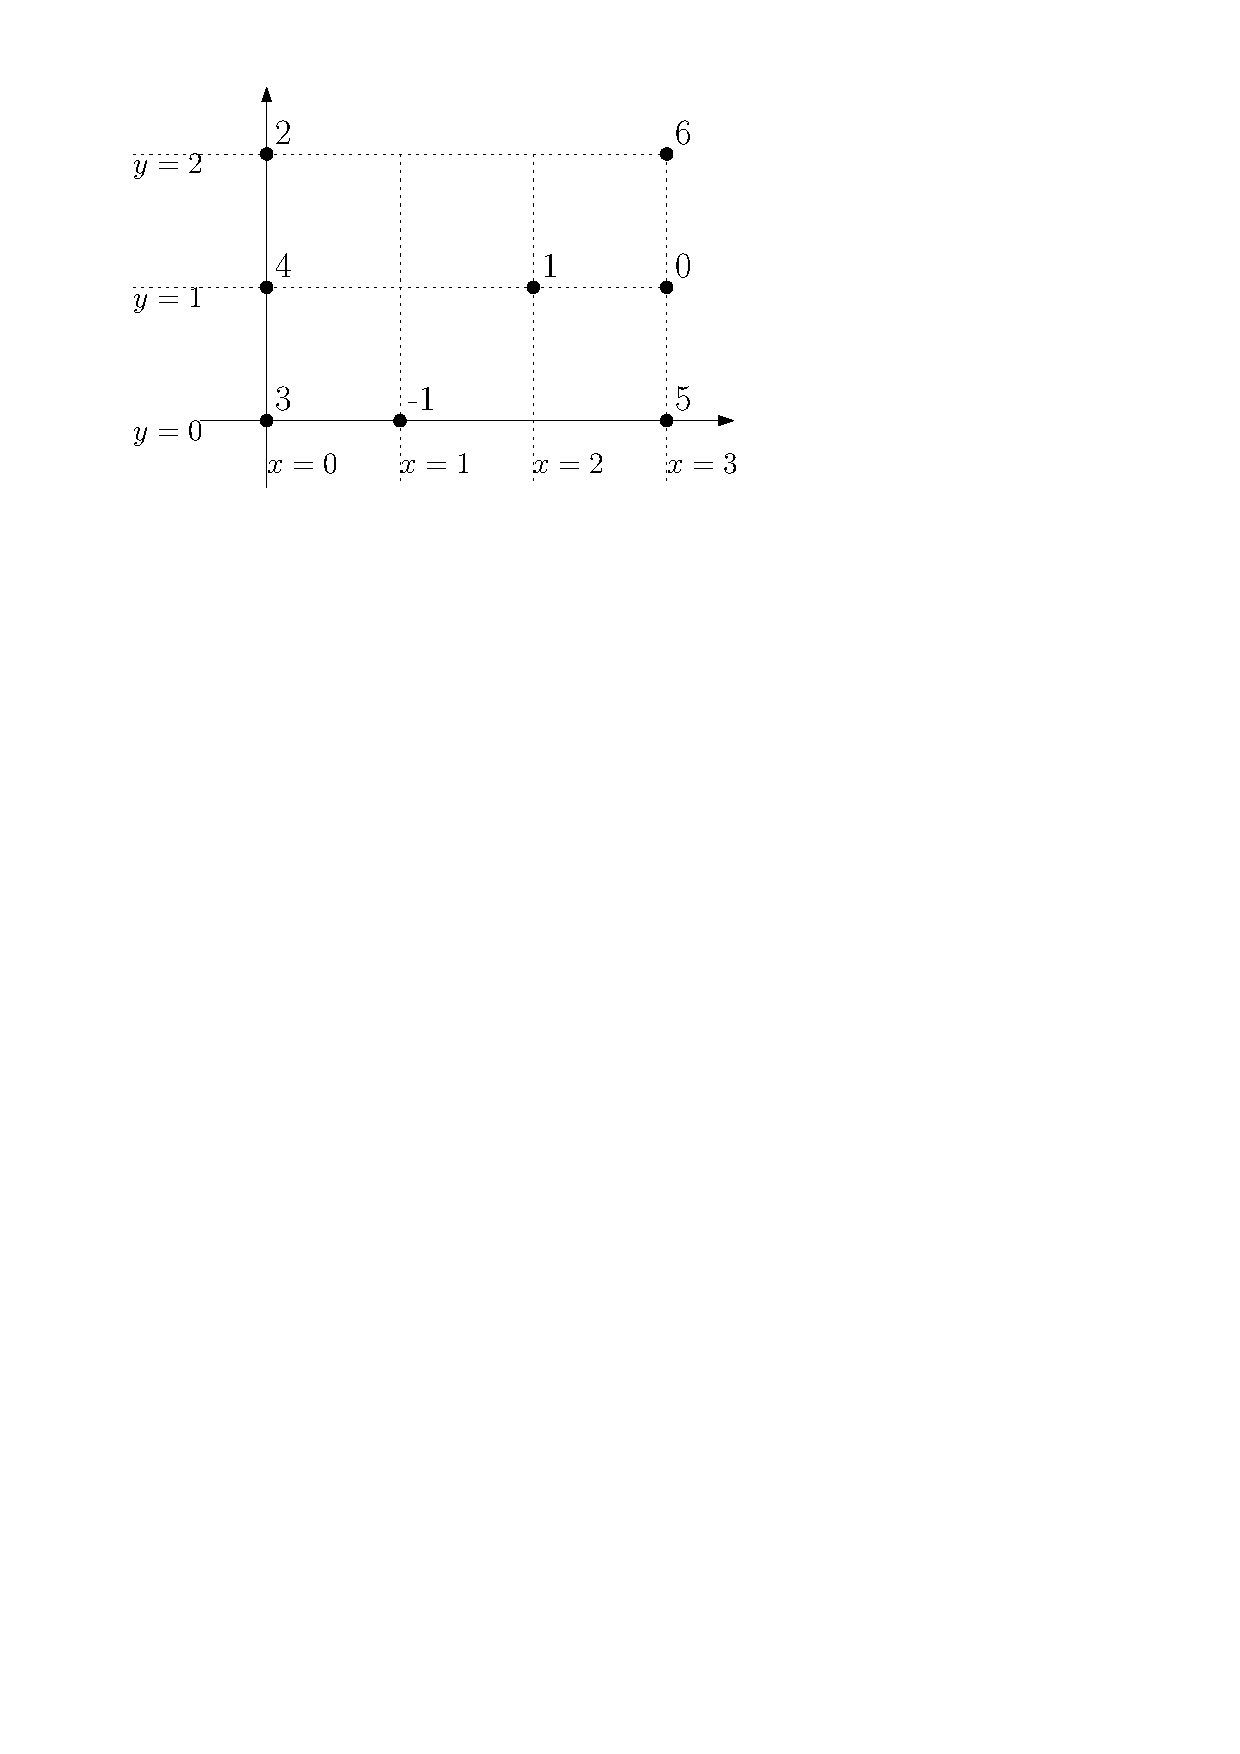
\includegraphics[width = .6\textwidth]{double.pdf}
\label{fig:double}
\end{figure}
\vfill
\pagebreak

\item (4 points) Write a MATLAB function that takes input
{\tt a, b} constants, and {\tt f} a function, and gives
as output an approximation
\[ \int_a^b f(x) \mathrm{dx}
\]
using three-point Gauss Quadrature. Note that the evaluation points and
weights are:

\begin{center}
\begin{tabular}{lccc}
  Evaluation points & $-\sqrt{3/5}$ & 0 & $\sqrt{3/5}$ \\
  Weights & $5/9$ & $8/9$ & $5/9$ \\
\end{tabular}
\end{center}
\end{document}
